%
% main.tex -- Paper zum Thema <francis>
%
% (c) 2020 Hochschule Rapperswil
%
\newcommand{\norm}[1]{\left\lVert#1\right\rVert}

\chapter{Francis Algorithmus\label{chapter:francis}}
\lhead{Francis-Algorithmus}
\begin{refsection}
\chapterauthor{Tobias Grab}

\begin{figure}
	\begin{center}
		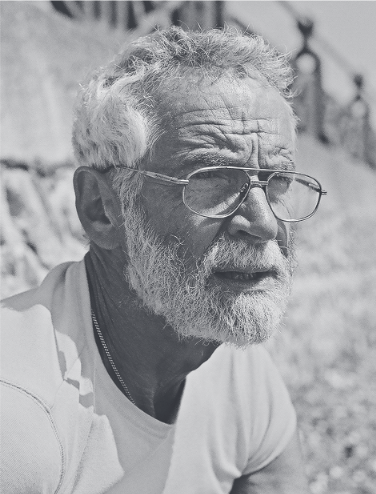
\includegraphics[scale=0.5]{papers/francis/images/Francis.png}
		\caption{John Francis im July 2008 \cite{francis:francis_portrait}}
		\label{John Francis}
	\end{center}
\end{figure}

Die Berechnung der Eigenvektoren und Eigenwerten einer Matrix ist in der Wissenschaft ein sehr oft vorkommendes Problem.
Mittlerweile halten wir die Berechnung für selbstverständlich.
Dank guter Hardware und vor allem guter Software ist das heutzutage meist kein Problem mehr, auch nicht von grossen Matrizen.
Eine effiziente Berechnung ist in vielen Bibliotheken integriert, wie beispielsweise der MATLAB-Befehl \glqq eig \grqq.
Vor rund 60 Jahren sah die Situation völlig anders aus.
Zum einen war die zur Verfügung stehende Hardware langsam und unzuverlässig, aber vor allem kannte niemand einen zuverlässig und effizienten Weg zur Berechnung.
Dies änderte sich im Jahre 1959 also John Francis den implizit geshifteten QR-Algorithmus, heute auch bekannt unter dem Namen \glqq Francis Algorithmus \grqq, entwickelt und verifiziert hat.
Der Algorithmus bzw. verschiedene Versionen davon werden bis heute von diversen Bibliotheken benutzt. \cite{francis:watkins_paper}

Wieso wird zur Berechnung der Eigenvektoren ein numerisches Verfahren benötigt?
Zur Berechnung der Eigenwerte einer 3x3 Matrix kann man das charakteristische Polynom bilden und dessen Nullstellen finden, diese entsprechen den Eigenwerten der Matrix.
Das Grundlegende Problem ist also die Suche nach den Nullstellen eines Polynoms.
Anfangs des 19. Jahrhunderts wurde von Niels Henrik Abel bewiesen, dass es keine Formel zur Berechnung der Nullstellen eines Polynoms der 5. Ordnung gibt.
Folglich ist auch eine direkte Berechnung der Eigenwerte einer Matrix nicht möglich und die numerische Berechnung mit einem iterativen Verfahren der einzige Weg.

\section{Grundlagen\label{francis:section:grundlagen}}
\rhead{Grundlagen}
Um ein besseres Verständnis für den Algorithmus zu bekommen, wollen wir uns zuerst einige wichtige Resultate aus der linearen Algebra in Erinnerung rufen.

\subsection{Ähnlichkeitstransformation\label{francis:section:grundlagen:aehnlichkeitstransform}}
Wird eine Matrix von rechts mit einer Matrix $C$ multipliziert und von links mit der Inversen $C^{-1}$, handelt es sich um eine Ähnlichkeitstransformation. Die Transformation ist auch bekannt als Basiswechsel bzw. Similarity Transformation
\begin{equation}
	\hat{A}=C^{-1}AC.
\end{equation}
Oft wird die Transformation auch in der Form $C\hat{A}=AC$ dargestellt, welche sich durch einfaches Umformen erreichen lässt.
Es handelt sich bei einer solchen Transformation lediglich um einen Wechsel des Koordinatensystems.
Daher sind einige Eigenschaften einer Matrix gegenüber einer solchen Transformation invariant.
Zueinander ähnliche Matrizen haben:
\begin{enumerate}
	\item die gleiche Determinante
	\item die gleiche Spur
	\item den gleichen Rang
	\item das gleiche Minimalpolynom
	\item die gleiche jordanische Normalform
	\item \textbf{die gleichen Eigenwerte (aber nicht notwendigerweise die gleichen Eigenvektoren)}
\end{enumerate}

Eigenwerte und Eigenvektoren können gefunden werden, indem man eine Matrix durch Ähnlichkeitstransformation auf Diagonalform bringt.
Der Francis-Algorithmus tut dies Schrittweise unter Verwendung sehr spezieller Matrizen $C$.

\subsection{Spezielle Matrizen\label{francis:section:grundlagen:spezielle_matrizen}}
Im Folgenden werden wir immer wieder über einige spezielle Matrixformen sprechen.
Reden wir von einer Matrix in der oberen Hessenberg-Form, meinen wir eine Matrix der Form:
\begin{equation}
	\begin{bmatrix}
	* & * & * & * & * \\
	* & * & * & * & * \\
	& * & * & * & * \\
	&   & * & * & * \\
	&   &   & * & *
	\end{bmatrix},
\end{equation}
wobei die Sterne bedeuten, dass an dieser Stelle ein Wert in der Matrix steht, welcher nicht Null ist.
Die Form entspricht also fast einer oberen Dreiecksmatrix, zusätzlich sind aber alle Elemente unmittelbar unter der Diagonalen von Null verschieden.
Mit dem weiter unten im Abschnitt \ref{francis:section:vorbereitung} vorgestellten Verfahren kann eine allgemeine Matrix in obere Hessenberg-Form gebracht werden. Wendet man das gleiche Verfahren aber auf eine symmetrische Matrix an, entsteht eine Spezialform, eine Tridiagonalmatrix:

\begin{equation}
	\begin{bmatrix}
	* & * &   &   &   \\
	* & * & *  &   &   \\
	& * & * & * &  \\
	&   & * & * & * \\
	&   &   & * & *
	\end{bmatrix}.
\end{equation}

\subsection{Eigenwerte\label{francis:section:grundlagen:eigenwerte}}
Bei den Eigenvektoren einer Matrix handelt es sich um Vektoren, welche bei einer Multiplikation mit der Matrix die Richtung nicht ändern, sondern lediglich gestreckt werden.

\begin{satz}
	Ein Vektor $v$ $\subset \mathbb{C}^n$ ist ein Eigenvektor von A, wenn v $\neq$ und $Av$ ein Vielfaches von $v$ ist. Der Skalar $\lambda$ ist der zum Eigenvektor $v$ gehörende Eigenwert von $A$
\end{satz}

Es gilt also:
\begin{equation}
	Av=\lambda v.
\end{equation}
Gesucht sind die Nullstellen des charakteristischen Polynoms

\begin{equation}
	\chi_A(\lambda)=\det(A-\lambda I) = 0.
\end{equation}
 Da ein Polynom vom Grad $n$ höchstens $n$ Nullstellen hat, gibt es auch höchstens $n$ Eigenwerte.

\begin{beispiel}
Die Eigenwerte einer kleinen Matrix
	\begin{equation}
	A =
	\begin{bmatrix}
	1 & 3 & 2 \\
	0 & 2 & 1 \\
	0 & 0 & 3
	\end{bmatrix}
	\end{equation}
können wie folgt berechnet werden.
	
	\begin{equation}
	\det(A-\lambda I)= \det
	\begin{pmatrix}
	\begin{bmatrix}
	1-\lambda & 3 & 2 \\
	0 & 2-\lambda & 1 \\
	0 & 0 & 3-\lambda
	\end{bmatrix}
	\end{pmatrix}
	= 0
	\end{equation}	
daraus folgt:
	
	\begin{equation} 
	(1-\lambda)(2-\lambda)(3-\lambda)=0
	\end{equation}
und die Eigenwerte sind mit $\lambda_{1}=1$, $\lambda_{2}=2$ und $\lambda_{3}=3$ gefunden.
\end{beispiel}

Wie im Beispiel ersichtlich, sind die Eigenwerte einer Matrix in Dreiecks- oder Diagonalform durch die Diagonalelemente gegeben.
Da bei Bestimmung der Determinante (bei 3. Ordnung z. B. mit der Regel von Sarrus) alles andere verschwindet.

\subsection{Givens-Rotationen\label{francis:section:grundlagen:givens}}
Rotationsmatrizen sind attraktiv, da sie einfach konstruiert werden können und mit ihnen durch eine geeignete Wahl des Rotationswinkels an einer gewünschten Stelle in einem Vektor eine Null erzeugt werden kann.
Dazu wird eine Rotations- bzw. Drehmatrix verwendet.
Sie hat in zwei Dimensionen die folgende Form:
\begin{equation}
	R=\begin{bmatrix}
	\cos\phi & -\sin\phi \\
	\sin\phi & \cos\phi
	\end{bmatrix}.
\end{equation}
Zur Drehung eines Punktes $P=(x,y)$ um den Winkel $\phi$ kann man einfach den dazugehörigen Ortsvektor mit der Rotationsmatrix multiplizieren und erhält so den Ortsvektor des gedrehten Punktes.
Es handelt sich dabei um eine Givens-Rotationsmatrix, wenn $R^{-1}(\phi)=R_{T}(\phi)=R(-\phi)$.
Durch Erweiterung der Rotationsmatrix können Drehungen natürlich auch in einem höherdimensionalem Raum verwendet werden.

\begin{beispiel}
Gegeben sei die Multiplikation einer Rotationsmatrix mit einem beliebigen Vektor:
	\begin{equation}
	\begin{bmatrix}
	1 & 0 & 0 & 0 & 0 & 0 \\
	0 & \cos\phi & 0 & 0 & -\sin\phi & 0 \\
	0 & 0 & 1 & 0 & 0 & 0 \\
	0 & 0 & 0 & 1 & 0 & 0 \\
	0 & \sin\phi & 0 & 0 & \cos\phi & 0 \\
	0 & 0 & 0 & 0 & 0 & 1 \\
	\end{bmatrix}
	\begin{bmatrix}
	x_{1}\\
	x_{2}\\
	x_{3}\\
	x_{4}\\
	x_{5}\\
	x_{6}\\
	\end{bmatrix}
	=
	\begin{bmatrix}
	x_{1}\\
	x_{2}\cos\phi-x_{5}\sin\phi\\
	x_{3}\\
	x_{4}\\
	x_{2}\sin\phi+x_{5}\cos\phi\\
	x_{6}\\
	\end{bmatrix}.
	\end{equation}	
Wie dabei zu sehen ist, werden dabei nur die 2. und 5. Spalte des Vektors verändert.
Eine Anwendung einer solchen Rotationsmatrix entspricht also einer Rotation in jener Ebene im 6-dimensionalen Raum, welche von Achse 2 und 5 aufgespannt wird.
Durch eine geeignete Wahl des Rotationswinkels und ein systematisches Anwenden diverser Rotationsmatrizen kann man so einen Eintrag nach dem Andern auf Null setzen und beispielsweise eine QR-Zerlegung durchführen. \cite{francis:QR_Zerlegung} 
Weiteres dazu ist in den Kapiteln \ref{buch:section:qr} und \ref{chapter:qr} zu finden.
\end{beispiel}

\subsection{Householder-Transformation\label{francis:section:grundlagen:householder}}
Reflektoren (siehe Abschnitt \ref{buch:subsection:spiegelungn}) sind attraktiv, da sie einfach konstruiert werden können und mit ihnen alle Elemente eines Vektors bis auf ein Element auf Null gesetzt werden können.
So kann jede beliebige Matrix relativ einfach in Hessenberg-Form gebracht werden.
Ein beliebiger Vektor $x$ und ein spezieller Vektor $y$ sind gegeben.
\begin{equation}
	x=
	\begin{bmatrix}
	x_{1}\\
	x_{2}\\
	\vdots\\
	x_{n}\\
	\end{bmatrix}
	,\qquad y=
	\begin{bmatrix}
	y_{1}\\
	0\\
	\vdots\\
	0\\
	\end{bmatrix}, \text{mit } y_{1}\pm \norm{x}	
\end{equation}
Da diese beiden Vektoren dieselbe Länge haben, wissen wir, dass ein Reflektor $H$ existiert, sodass $Hx=y$.
Mit dem Reflektor
\begin{equation}
	H=I-2vv^{T}, \text{mit } v=(x-y)/\norm{x-y}
\end{equation}
können also alle Elemente eines Vektors bis auf ein Element auf null gesetzt werden.
Das Ganze ist in Abbildung \ref{francis:abb:householder_transform} in zwei Dimensionen dargestellt.
\begin{figure}[h]
	\begin{center}
		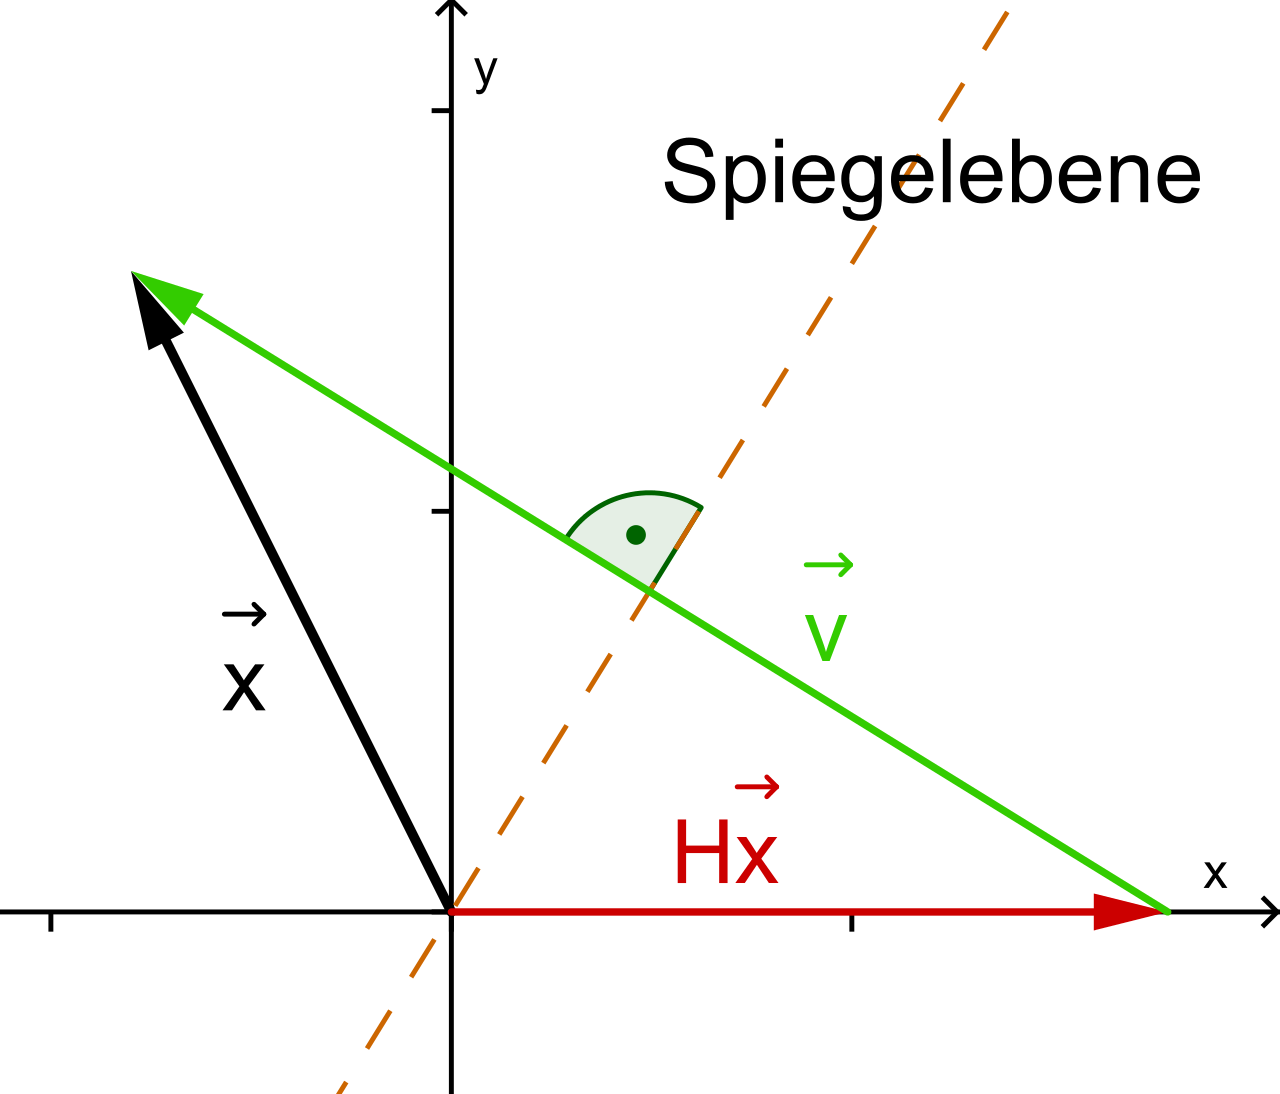
\includegraphics[scale=0.1]{papers/francis/images/Householdertransformation.png}
		\caption{Illustration der Householder-Transformation in zwei Dimensionen, Abbildung von \cite{francis:householder}}
		\label{francis:abb:householder_transform}
	\end{center}
\end{figure}

\section{Vorbereitung der Matrix\label{francis:section:vorbereitung}}
\rhead{Vorbereitung}
Um den Francis-Algorithmus effizient ausführen zu können, muss die Matrix zuerst auf Hessenberg-Form gebracht werden.
\begin{equation}
	\begin{bmatrix}
	* & * & * & * & * \\
	* & * & * & * & * \\
	*& * & * & * & * \\
	*&  * & * & * & * \\
	*&  * &  * & * & *
	\end{bmatrix} \rightarrow
	\begin{bmatrix}
	* & * & * & * & * \\
	* & * & * & * & * \\
	& * & * & * & * \\
	&   & * & * & * \\
	&   &   & * & *
	\end{bmatrix}
\end{equation}

\begin{satz}
	Jede Matrix $ A \subset \mathbb{R} ^{n \times n} $ ist orthogonal ähnlich zu einer Matrix H in der oberen Hessenberg-Form: $ H=Q^{-1}AQ $, wobei $Q$ ein Produkt von $n-2$ Reflektoren ist.
\end{satz}

Gegeben sei eine Matrix A mit einer Submatrix $\hat{A}$, einer ersten Spalte $a_{11}$ und einem Vektor $b$.
\begin{equation}
A=
\begin{bmatrix}
a_{11} & *\\
b & \hat{A}
\end{bmatrix}.
\end{equation}
Ziel ist es, alle Einträge dieses Vektors bis auf den Ersten auf Null zu setzen.
Dies kann mit einer Multiplikation mit einer geeigneten Matrix
\begin{equation}
Q_{1}=
\begin{bmatrix}
	1 & *\\
	0 & \hat{Q}_1
\end{bmatrix}
\end{equation}
gemacht werden.
$\hat{Q}_1$ muss so gewählt werden, dass bei einer Multiplikation mit $b$ alle Werte bis auf den Ersten verschwinden.
Zusätzlich soll die Länge des neuen Vektors $\hat{Q}_1b$, bzw. dieser einzelne Eintrag, der Länge des Vektors $b$ entsprechen:
\begin{equation}
\hat{Q}_1b=
\begin{bmatrix}
-y\\
0\\
\vdots\\
0
\end{bmatrix}.
\end{equation}
Wird $\hat{Q}_1$ so gewählt, entsteht bei einer Multiplikation von links mit der Matrix $Q_1$ der gewünschte Vektor in der ersten Spalte.
\begin{equation}
A_{\text{Half}}=Q_{1}A=
\begin{bmatrix}
a_{11} & * & \dots & *\\
-y & \\
0 & & & &\\
\vdots & &\hat{Q}_1\hat{A} & &\\
 & & & &\\
0 & & & &
\end{bmatrix}
\end{equation}
$\hat{Q}_1$ kann dabei zum Beispiel mit Givens Rotationsmatrizen \ref{francis:section:grundlagen:givens} oder einer Householder-Trans\-for\-ma\-tions\-ma\-trix \ref{francis:section:grundlagen:householder} gebildet werden.

Damit wir die Eigenwerte unserer Matrix nicht verändern, müssen wir die Matrix $Q_1$ nun auch von der rechten Seite hinzu multiplizieren.
Da die erste Spalte von $Q_1$ nur eine Eins und sonst Nullen hat, wird dabei die vorher erzeugte Spalte nicht beeinflusst.
Das Resultat ist also eine ähnliche Matrix
\begin{equation}
	A_{1}=A_{\text{Half}}Q_{1}=
	\begin{bmatrix}
	a_{11} & * & \dots & *\\
	-y & \\
	0 & & & &\\
	\vdots & &\hat{Q}_1\hat{A}\hat{Q}_1^{-1} &\\
	 & & & &\\
	0 & & & &
	\end{bmatrix}
	=
	\begin{bmatrix}
	a_{11} & * & \dots & *\\
	-y & \\
	0 & & & &\\
	\vdots & &\hat{A}_{-1} &\\
	 & & & &\\
	0 & & & &
	\end{bmatrix},
\end{equation}	
welche an den gewünschten Stellen in der ersten Spalte Nullen hat.

Das gleiche Prinzip wird jetzt auf die Submatrix angewendet.
Durch den zweiten Reflektor entstehen Nullen in der zweiten Spalte:
\begin{align*}
	Q_{2}&=
	\begin{bmatrix}
	1 & 0 & 0 & \dots & 0\\
	0 & 1 & 0 & \dots & 0\\
	0 & 0 &\\
	\vdots & \vdots & &\hat{Q}_2 &\\
	 &  &\\
	0 & 0 &
	\end{bmatrix},
&&&
	A_{2}&=
	\begin{bmatrix}
	a_{11} & * &  & \dots & *\\
	-y_{1} & * &  & \dots & *\\
	0 & -y_{2} &\\
	\vdots & \vdots  & &\hat{Q}_2\hat{A}_{2}\hat{Q}_2^{-1} &\\
	 &  &\\
	0 & 0 &
	\end{bmatrix}.
\end{align*}
Mit einem weiteren Schritt ebenfalls in der dritten Spalte usw.
Das Resultat ist eine Matrix in der Hessenberg-Form, welche ähnlich zu $A$ ist.
Das heisst für uns, sie besitzt dieselben Eigenwerte wie die Matrix $A$.
Die ganzen Multiplikation der Reflektoren kann zusammengefasst werden, sodass sich eine einzige Ähnlichkeitstransformation
\begin{equation}
	H=Q_{n-2}Q_{n-1}\dots Q_{1}AQ_{1}^{-1}\dots Q_{n-1}^{-1}Q_{n-2}^{-1}
\end{equation}
ergibt.
Mit 
\begin{equation}
	Q=Q_{1}\dots Q_{n-1}Q_{n-2}
\end{equation}
erhalten wir
\begin{equation}
	Q^{-1} = Q_{n-2}^{-1}Q_{n-1}^{-1}\dots Q_{1}^{-1}
\end{equation}
und schlussendlich
\begin{equation}
H=Q^{-1}AQ.
\end{equation}

Im Falle einer symmetrischen Matrix $A$ werden durch die Multiplikation von rechts dieselben Elemente im oberen Teil der Matrix eliminiert und das Ergebnis der Transformation ist tridiagonal.
Durch die Reduzierung der ursprünglichen Matrix auf Hessenberg-Form, werden die Kosten des anschliessenden Algorithmus stark reduziert.

\section{Francis Iteration erster Ordnung\label{francis:section:francis_iteration}}
\rhead{Francis Iteration erster Ordnung}

Nun wollen wir uns mit dem eigentlichen Francis Algorithmus \cite{francis:watkins_book} befassen.
Es handelt sich dabei um ein iteratives Verfahren und lässt sich daher am besten durch die Analyse einer Iteration beschreiben.
Die Ausgangssituation für den Algorithmus ist eine Matrix, welche sich in oberer Hessenberg Form oder sogar tridiagonaler Form befindet.

Der Algorithmus beginnt mit der Wahl eines Shifts $\rho_{1}$ und der Berechnung der ersten Spalte von $A-\rho_{1} I$. 
Diese hat die Form
\begin{equation}
	p=\begin{bmatrix}
	a_{11}-\rho_{1}\\
	a_{21}\\
	0\\
	\vdots\\
	\\
	0
	\end{bmatrix}.
\end{equation}

Anschliessend muss eine Matrix $Q_{0}$ gefunden werden, welche auf den Achsen 1 und 2 arbeitet und den Wert von $a_{21}$ eliminiert. Diese kann zum Beispiel mit Givens Rotationsmatrizen \ref{francis:section:grundlagen:givens} oder einer Householder-Transformationsmatrix \ref{francis:section:grundlagen:householder} gebildet werden.

\begin{equation}
	Q_{0}^{-1}p=\begin{bmatrix}
	*\\
	0\\
	0\\
	\vdots\\
	\\
	0
	\end{bmatrix}
\end{equation}

Danach muss $A$ mit $Q_{0}$ zu  $Q_{0}^{-1}AQ_{0}$ transformiert werden.
Die Transformation von $A$ nach $Q_{0}^{-1}A$ kombiniert lediglich die Zeilen 1 und 2, die Matrix behält aber ihre Hessenberg Form.
Die anschliessende Transformation von $Q_{0}^{-1}A$ nach $Q_{0}^{-1}AQ_{0}$ kombiniert die Spalten 1 und 2, wodurch die Hessenberg Form zerstört wird.
Es entsteht an der Stelle (3,1) eine "`Ausbuchtung"'.
Der Rest der Iteration beschäftigt sich damit, die Matrix wieder in ihre Hessenberg Form zu bringen.
Dafür wählen wir eine Matrix welche auf den Achsen 2 und 3 arbeitet und den Wert von $a_{31}$ eliminiert.
So wird die Ausbuchtung nach unten verschoben.
Dieses Prozedere wird wiederholt, bis die Ausbuchtung schlussendlich unten aus der Matrix hinausgeschoben wird.
Die Hessenberg Form ist wiederhergestellt.

Bei einer $5 \times 5$ Matrix sieht eine Iteration also wie folgt aus:
\begin{equation}
	\begin{bmatrix}
	* & * & * & * & *  \\
	* & * & *  & * & *  \\
	+ & * & * & * & *\\
	&   & * & * & * \\
	&   &   & * & * 
	\end{bmatrix} \rightarrow
	\begin{bmatrix}
	* & * & * & * & *  \\
	* & * & *  & * & *  \\
	& * & * & * & *\\
	&  + & * & * & * \\
	&   &   & * & * 
	\end{bmatrix} \rightarrow
	\begin{bmatrix}
	* & * & * & * & *  \\
	* & * & *  & * & *  \\
	& * & * & * & *\\
	&   & * & * & * \\
	&   &  + & * & * 
	\end{bmatrix} \rightarrow
	\begin{bmatrix}
	* & * & * & * & *  \\
	* & * & *  & * & *  \\
	& * & * & * & *\\
	&   & * & * & * \\
	&   &   & * & * 
	\end{bmatrix}
\end{equation}

Das Resultat einer Francis Iteration ist also
\begin{equation}
	\hat{A}=Q_{n-2}\dots Q_{1}Q_{0}AQ_{0}^{-1}Q_{1}^{-1}\dots Q_{n-2}^{-1},
\end{equation}
wobei $Q_{0}$ die Transformation bezeichnet, welche eine Ausbuchtung in der Matrix erzeugt und $Q_{1},\dots,Q_{n-2}$ die Transformationen sind, welche die Hessenberg Form wiederherstellen.
Dabei handelt es sich also nur um Ähnlichkeitstransformationen und $\hat{A}$ besitzt dementsprechend die gleichen Eigenwerte wie $A$.
Mit jeder Iteration konvergieren die Elemente unter der Diagonalen weiter gegen null und die Eigenwerte erscheinen dementsprechend auf der Diagonalen von $\hat{A}$.

\subsection{Wahl der Shifts\label{francis:section:francis_iteration:wahl_shift}}
Die Shifts werden zur Konvergenzbeschleunigung gebraucht.
Die Wahl eines guten Shifts kann den Algorithmus drastisch beschleunigen. 
Ein guter Shift ist dabei einer, welcher einen Eigenwert der Matrix gut approximiert.

Unser Algorithmus verkleinert bei jeder Iteration die Elemente auf der Subdiagonalen.
Die Diagonalelemente werden daher eine immer bessere Approximationen der Eigenwerte.
Daher wird oft ein Eigenwert auf der Diagonalen als Shift für die nächste Iteration verwendet.
Zu Beginn mag dies noch eine schlechte Approximation sein, sie verbessert sich aber sehr schnell.

Wird das unterste Diagonalelement verwendet spricht man von einem Rayleigh-Quotienten-Shift.
Eine andere, ähnliche Shift-Strategie ist der nach James Hardy Wilkinson benannte Wilkinson-Shift.
Für diesen wird der näher am letzten Matrixelement liegende Eigenwert der untersten "`$2\times2$ Matrix"' als Shift benutzt.


\begin{beispiel}
	Gegeben sei eine Matrix $A$, welche sich bereits in Hessenberg Form befindet
	
	\begin{equation}
	A=
	\begin{bmatrix}
	17 & -28.941 & 1.847 & -4.46 & 2.257\\
	-27.677 & 33.94 & 26.188 & -2.228 & 1.268\\
	0 & 25.096 & 20.687 & -6.606 & -0.197\\
	0 & 0 & -5.963 & \textcolor{orange}{-16.816} & \textcolor{orange}{-12.445}\\
	0 & 0 & 0 & \textcolor{orange}{-9.01} & \textcolor{red}{10.189}\\
	\end{bmatrix} 
	\qquad
	\text{mit }
	\texttt{eig}(A)=
	\begin{bmatrix}
	65 & \\
	-21.277 & \\
	-13.126 & \\
	21.277 & \\
	13.126 & \\
	\end{bmatrix}
	\end{equation}
	
	Für die den Rayleigh-Quotienten-Shift-Strategie würde man also \textcolor{red}{$10.189$} als ersten Shift verwenden.
	Verfolgt man die Wilkinson-Shift-Strategie, würde man die Eigenwerte der Matrix

	\begin{equation}
	\begin{bmatrix}
	 \textcolor{orange}{-16.816} & \textcolor{orange}{-12.445}\\
	 \textcolor{orange}{-9.01} & \textcolor{red}{10.189}\\
	\end{bmatrix}
	\end{equation}
	berechnen.
	Dabei findet man $-21.279$ und $13.126$.
	Da $13.126$ näher als $-21.279$ am untersten Diagonalelement liegt, wird dies als erster Shift verwendet.
	Dabei handelt es sich schon um eine gute Annäherung für einen Eigenwert der Matrix $A$.	
\end{beispiel}



\section{Francis Iteration der Ordnung n}
\rhead{Francis Iteration der Ordnung n}

Im Prinzip kann eine Francis Iteration für eine beliebige Ordnung n durchgeführt werden, praktisch sollte die Ordnung n aber klein gewählt werden.
Francis hat die Ordnung n=2 gewählt.
Gegenüber der Ordnung n=1 entsteht dabei der Vorteil, dass für komplex konjugierte Shifts gewählt werden können (Und somit auch komplex konjugierte Eigenwerte approximiert) ohne dass komplex gerechnet werden muss.

Berechnung einer Francis Iteration:
\begin{enumerate}
	\item Wähle n verschiedene Shifts $\rho_{1}$ ... $\rho_{n}$.
	\item Berechne $p= (A - \rho_{n}I) ... (A - \rho_{1}I)e_{1}$.
	\item Berechne den Reflektor $Q_{0}$ dessen erste Kolonne proportional zu x ist.
	\item Führe eine Ähnlichkeitstransformation mit dem berechneten Shift $Q_{0}^{-1}AQ_{0}$, was eine \glqq Ausbuchtung \grqq in der Matrix erzeugt.
	\item Führe weitere Ähnlichkeitstransformationen durch, wobei sich die Ausbuchtung immer weiter nach unten verschiebt und sich schlussendlich wieder eine Hessenberg Matrix ergibt.
\end{enumerate}

Wichtig anzumerken ist, dass wir nach der Wahl von n Shifts nicht die gesamte Matrix $(A - \rho_{n}I) ... (A - \rho_{1}I)$ berechnen, denn die Kosten dafür wären zu hoch. Es reicht die erste Kolonne zu berechnen, welche bei einer vernünftigen Wahl von n einfach zu berechnen ist.

Der Francis Algorithmus der 1. Ordnung kann auf generelle komplexe Matrizen angewendet werden, wobei dann die ganze Arithmetik ebenfalls komplex ist.
Ist die Matrix und die Shifts aber real, so kann die ganze Iteration in reeller Arithmetik ausgeführt werden.
Beim Francis Algorithmus der 2. Ordnung können sogar konjugiert komplexe Shifts verwendet werden, aber die ganze Berechnung kann in reeller Arithmetik ausgeführt werden.
Die totalen Kosten für den expliziten QR Algorithmus für k Iterationen ist $8kn^{3}$ Additionen und $12kn^{3}$ Multiplikationen.
Im Vergleich dazu betragen die totalen Kosten für den impliziten QR Algorithmus (Francis) für k Iterationen ist $2kn^{3}$ Additionen und $2kn^{3}$ Multiplikationen, wobei ein Schritt des impliziten Verfahrens zwei Schritten des expliziten Verfahrens entspricht. \cite{francis:EthSeminar}

\section{Wieso der Algorithmus funktioniert\label{francis:section:wieso_es_funktioniert}}
\rhead{Wieso der Algorithmus funktioniert}


\printbibliography[heading=subbibliography]
\end{refsection}
